\section{The Dataset in This Repository}
\label{sec:dataset}

\subsection{Where the data lives}
The repository holds no folder of raw CIC-DDoS2019 CSVs. All data is in one 33\,MB file,
\code{output.csv}, which \code{main.py} reads through \code{data\_loader.load\_csv()} (default path
\code{./output.csv}). It has 74{,}999 data lines and 88 columns: an index column
(\code{Unnamed: 0}), seven identifier columns (\code{Flow ID}, source/destination IP and port,
\code{Protocol}, \code{Timestamp}), 77 numeric CICFlowMeter features, \code{SimillarHTTP},
\code{Inbound} and \code{Label}.

\paragraph{Provenance.} Several clues show how the file was made. Four of its lines repeat the
header row (with \code{Label}=``Label''), so it is a concatenation of several CICFlowMeter CSVs.
The class names (\code{MSSQL}, \code{LDAP}, \code{Portmap}, \code{Syn}, \code{UDP}, without the
\code{DrDoS\_} prefix used in the January files) and the presence of \code{Portmap} match the
CSVs of the \emph{11 March} capture day, whose timestamps read \code{2018-11-03}. The paper
attributes these classes to the 12 January ``training day''; that should be corrected. Each attack
class contributes roughly 10--20k rows (Table~\ref{tab:dups}), and the \code{Unnamed: 0} index
values (up to 482{,}780) point back to positions in much larger source files. Most importantly,
each class covers a \emph{very short time window}: all 14{,}999 \code{Syn} flows fall within
1.1\,s, all \code{UDP} flows within 2\,s, and all \code{LDAP} flows within about 2 minutes. The
file is therefore a set of contiguous slices from each class's capture, not a random sample of
the full dataset.

\subsection{Class composition and duplicates}
After removing the four repeated header lines, 74{,}995 rows remain. The loader counts two rows
as duplicates when all 61 feature columns used by the paper and the label are equal. By that
definition, \textbf{49{,}393 rows (65.9\%) are exact duplicates} of an earlier row
(Table~\ref{tab:dups}).

\begin{table}[H]
\centering\small
\caption{Rows, duplicates and unique rows per class in \code{output.csv} (paper feature set).}
\label{tab:dups}
\begin{tabular}{lrrrr}
\toprule
Class & Rows & Duplicates & Unique & Duplicate share \\
\midrule
BENIGN & 5,126 & 786 & 4,340 & 15.3\% \\
LDAP & 9,931 & 9,353 & 578 & 94.2\% \\
MSSQL & 19,657 & 13,697 & 5,960 & 69.7\% \\
Portmap & 10,284 & 9,521 & 763 & 92.6\% \\
Syn & 14,999 & 8,706 & 6,293 & 58.0\% \\
UDP & 14,998 & 7,330 & 7,668 & 48.9\% \\
\midrule
Total & 74,995 & 49,393 & 25,602 & 65.9\% \\

\bottomrule
\end{tabular}
\end{table}

The reflection attacks are almost entirely repetitive: only 578 of 9{,}931 LDAP flows and 763 of
10{,}284 Portmap flows are distinct. This is expected, since an amplification attack replays
the same request millions of times and CICFlowMeter maps identical packet trains to identical
feature vectors. It has a direct consequence for evaluation. If duplicates are kept and the data
is split at random, a large share of test flows have an identical copy in the training set, and
the classifier only needs to look them up. Section~\ref{sec:impdata} measures this effect:
about 30\% of test rows.

The low number of unique LDAP and Portmap flows also caps the balanced multiclass sample size.
With deduplication, the smallest class (LDAP, 578 unique flows) limits a balanced 6-class sample
to at most $6\times578=3468$ rows.

\subsection{Features}
The original loader lists 61 numeric columns (the ``paper'' feature set). Twelve are constant
zero in this file: \code{Bwd PSH Flags}, \code{Fwd/Bwd URG Flags}, \code{FIN}, \code{PSH} and
\code{ECE Flag Count}, and all six \code{Bulk} statistics. That leaves \textbf{49 informative
features}, not the 58 stated in the paper. The original loader padded the matrix with zero
columns to reach exactly 58; those columns carry no information and are dropped by PCA anyway.
The ``all'' feature set adds 16 more columns (Subflow counts, \code{Init\_Win\_bytes\_forward/backward},
\code{act\_data\_pkt\_fwd}, \code{min\_seg\_size\_forward}, Active/Idle statistics). Identifier
columns (IPs, ports, timestamps, flow IDs) are never used: in this testbed they would reveal the
attack hosts and time windows and give a trivially perfect but meaningless classifier.

The rate columns \code{Flow Bytes/s} and \code{Flow Packets/s} contain $\pm\infty$ in about 2{,}650
rows (CICFlowMeter divides by a zero duration). Five rows are NaN. Both are set to 0.

\paragraph{Heavy tails.} Most features are extremely skewed. \code{Flow Bytes/s} ranges up to
$2.9\times10^{9}$. Under linear min--max scaling to $[0,\pi]$, 35\% of flows receive an angle
below 0.01\,rad (Figure~\ref{fig:skew}). Across all 49 informative features, the median of the
90th percentile after min--max scaling is only $0.0017$: for 69\% of the features, nine out of ten
flows end up in the bottom 5\% of the rotation range. Section~\ref{sec:impdata} explains why this
matters for angle encoding and how a signed log transform fixes it.

\begin{figure}[H]
\centering
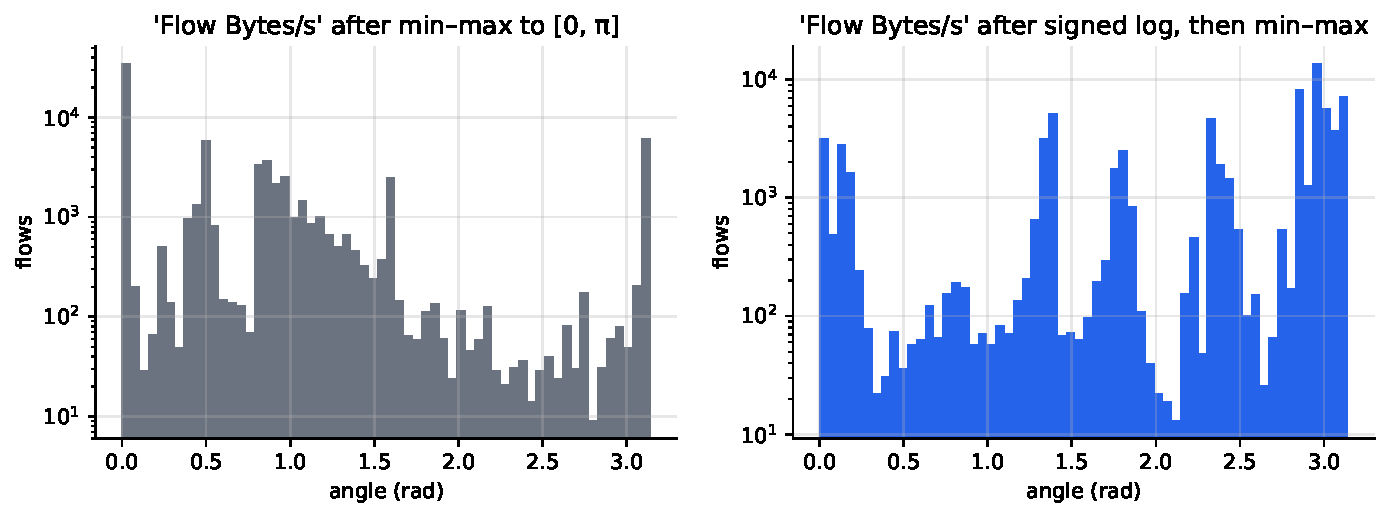
\includegraphics[width=\linewidth]{figures/skew.pdf}
\caption{Distribution of the rotation angle derived from \code{Flow Bytes/s} (log-scale
counts). Left: linear min--max, as in the original code; almost all mass sits at angle $\approx0$.
Right: after a signed $\log(1+|x|)$ transform the full $[0,\pi]$ range is used.}
\label{fig:skew}
\end{figure}

\subsection{Tasks}
\begin{itemize}
\item \textbf{Binary}: \code{BENIGN} (label 0) vs.\ any attack (label 1, ``DDoS''). Classes are
      balanced by undersampling. With deduplication the attack half is drawn from the pooled
      unique attack flows, which are dominated by UDP, Syn and MSSQL.
\item \textbf{Multiclass}: the six labels, BENIGN, LDAP, MSSQL, Portmap, Syn and UDP (alphabetical
      codes 0--5), undersampled to equal counts.
\end{itemize}
Both tasks use \code{--samples} (default 2000) as the total sample size, split 80/20 into
train/test with stratification. In multiclass mode that means 333 samples per class, 1{,}598
training samples and 400 test samples.
